%----------------------------------------------------------------------------
\chapter{The monitoring system}
%----------------------------------------------------------------------------
\section{Goal of the implementation}

After introducing the data formats and the cyberphisical system implementation, in this part a sample application is shown that can handle connection to both data types and visualize the measured data in an easily understandable format. This visualization should be viewable on all modern browsers including mobile phones and tablets.

The goal was to show how a connection can be created from third party applications and used as a transparent system. In further chapters the integration of the different types will be shown. The meaning of this phase is to seek for new ways to implement a web application using the connectors provided and measure the needs for such a web application. A whole test system has been created to enable this.

\section{The test environment}

The system has been tested on multiple platforms. There was an Ubuntu Linux based virtual machine, which had a limited 512 MB of RAM, and a max. 10 GB storage. It's network card was hidden behind a NAT provided by the host computer. Java Runtime Environment was installed on the virtual machine for Stardog and SOS. For the web application NodeJS has been set up. 

The other platform was a Windows based computer. It had the same services (Stardog and SOS) running. The monitoring application requires NodeJs, which is a platform independent solution, so this did not mean any problem. The Windows machine is located in the university and contains the SOS database with the real measurements provided by the sensors in the two locations described in the second use case. 

The chosen RDF database is Stardog Community edition. At first the software preallocates too much memory. It might be required for heavy weight applications but in our case it was not necessary.  The startup script had to be changed to make the software start. Changing this parameter does not decreases the performance significantly, compared to another computer with more memory. 

The chosen SOS server is 52north SOS 4.1 This is a recent release of the software. The used development version enables JSON communication. The server requires PostgreSQL database backend and Tomcat application server.

PostgreSQL 9.1.12 is used as the database backend for SOS. PostGIS environment had to be added. The database can be administrated using pgAdmin III from the host computer using port forward. For the Linux test environment no new users has been added, the SOS server uses the admin user to connect to the database. The database had to be created manually but tables and configuration is added during the installation automatically.

Tomcat 7 is installed to support SOS. To keep the system safe, on the Linux machine a new user is created to run the container and the application. The Stardog database is also running in a Tomcat like environment that is why it is started by the same user as the SOS server. 

\section{NodeJS: backend of the monitoring application}

The connector application is written in JavaScript. This way the frontend and the backend application can be written using the same programming language. 
Since the V8 engine exists JavaScript can be compiled and run significantly faster\cite{v8} than before. 
The engine was introduced in 2008 and it caused a breakthrough in Javascript language. It has some new solutions that made V8 more effective, these are:
\begin{itemize}
\item \textbf{Hidden classes}: In V8 every object is a class. They are stored in a tree based structure and can be recalled faster.
\item \textbf{Dynamic Machine Code Generation}: V8 generates machine code from source without any intermediate bytecode language, like in Java.
\item \textbf{Inline cache}: It has a built in inline cache for resolving method names quicker.
\item \textbf{Efficient Garbage Collection}:Garbage collection freezes code execution and has a detailed map of the variable, however each garbage collection phase would only clear some part of the memory, it does not run full garbage collection every time.
\end{itemize}
NodeJS builds upon this V8 engine and lets JavaScript run on backend. Another advantage is that NodeJS has a single threaded, event driven core. This enables running applications faster, without worrying about thread safety. The architecture of the NodeJS environment can be seen on figure \ref{fig:node}. 
To keep the integrator separated a different user is added to run server side code on the Linux system. 
No web application container or web server is needed to run a NodeJS application. 
The software itself handles TCP connections and other modules help do it similar to Java Servlets. 
Because it has smaller overhead and dependencies, the created application should run faster than a rich Java Web application. 
NodeJS has an easy to use packaging system that makes dependency handling simple, like maven for Java. All necessary modules names are added to the related part of the package.json file and required packages are downloaded using the npm install command from a central repository. On the Windows machine a fork of NodeJS, the IOJS engine was tested. It is a community driven alternative that is fully compatible with NodeJS.
 
\begin{figure}[h]
\centering
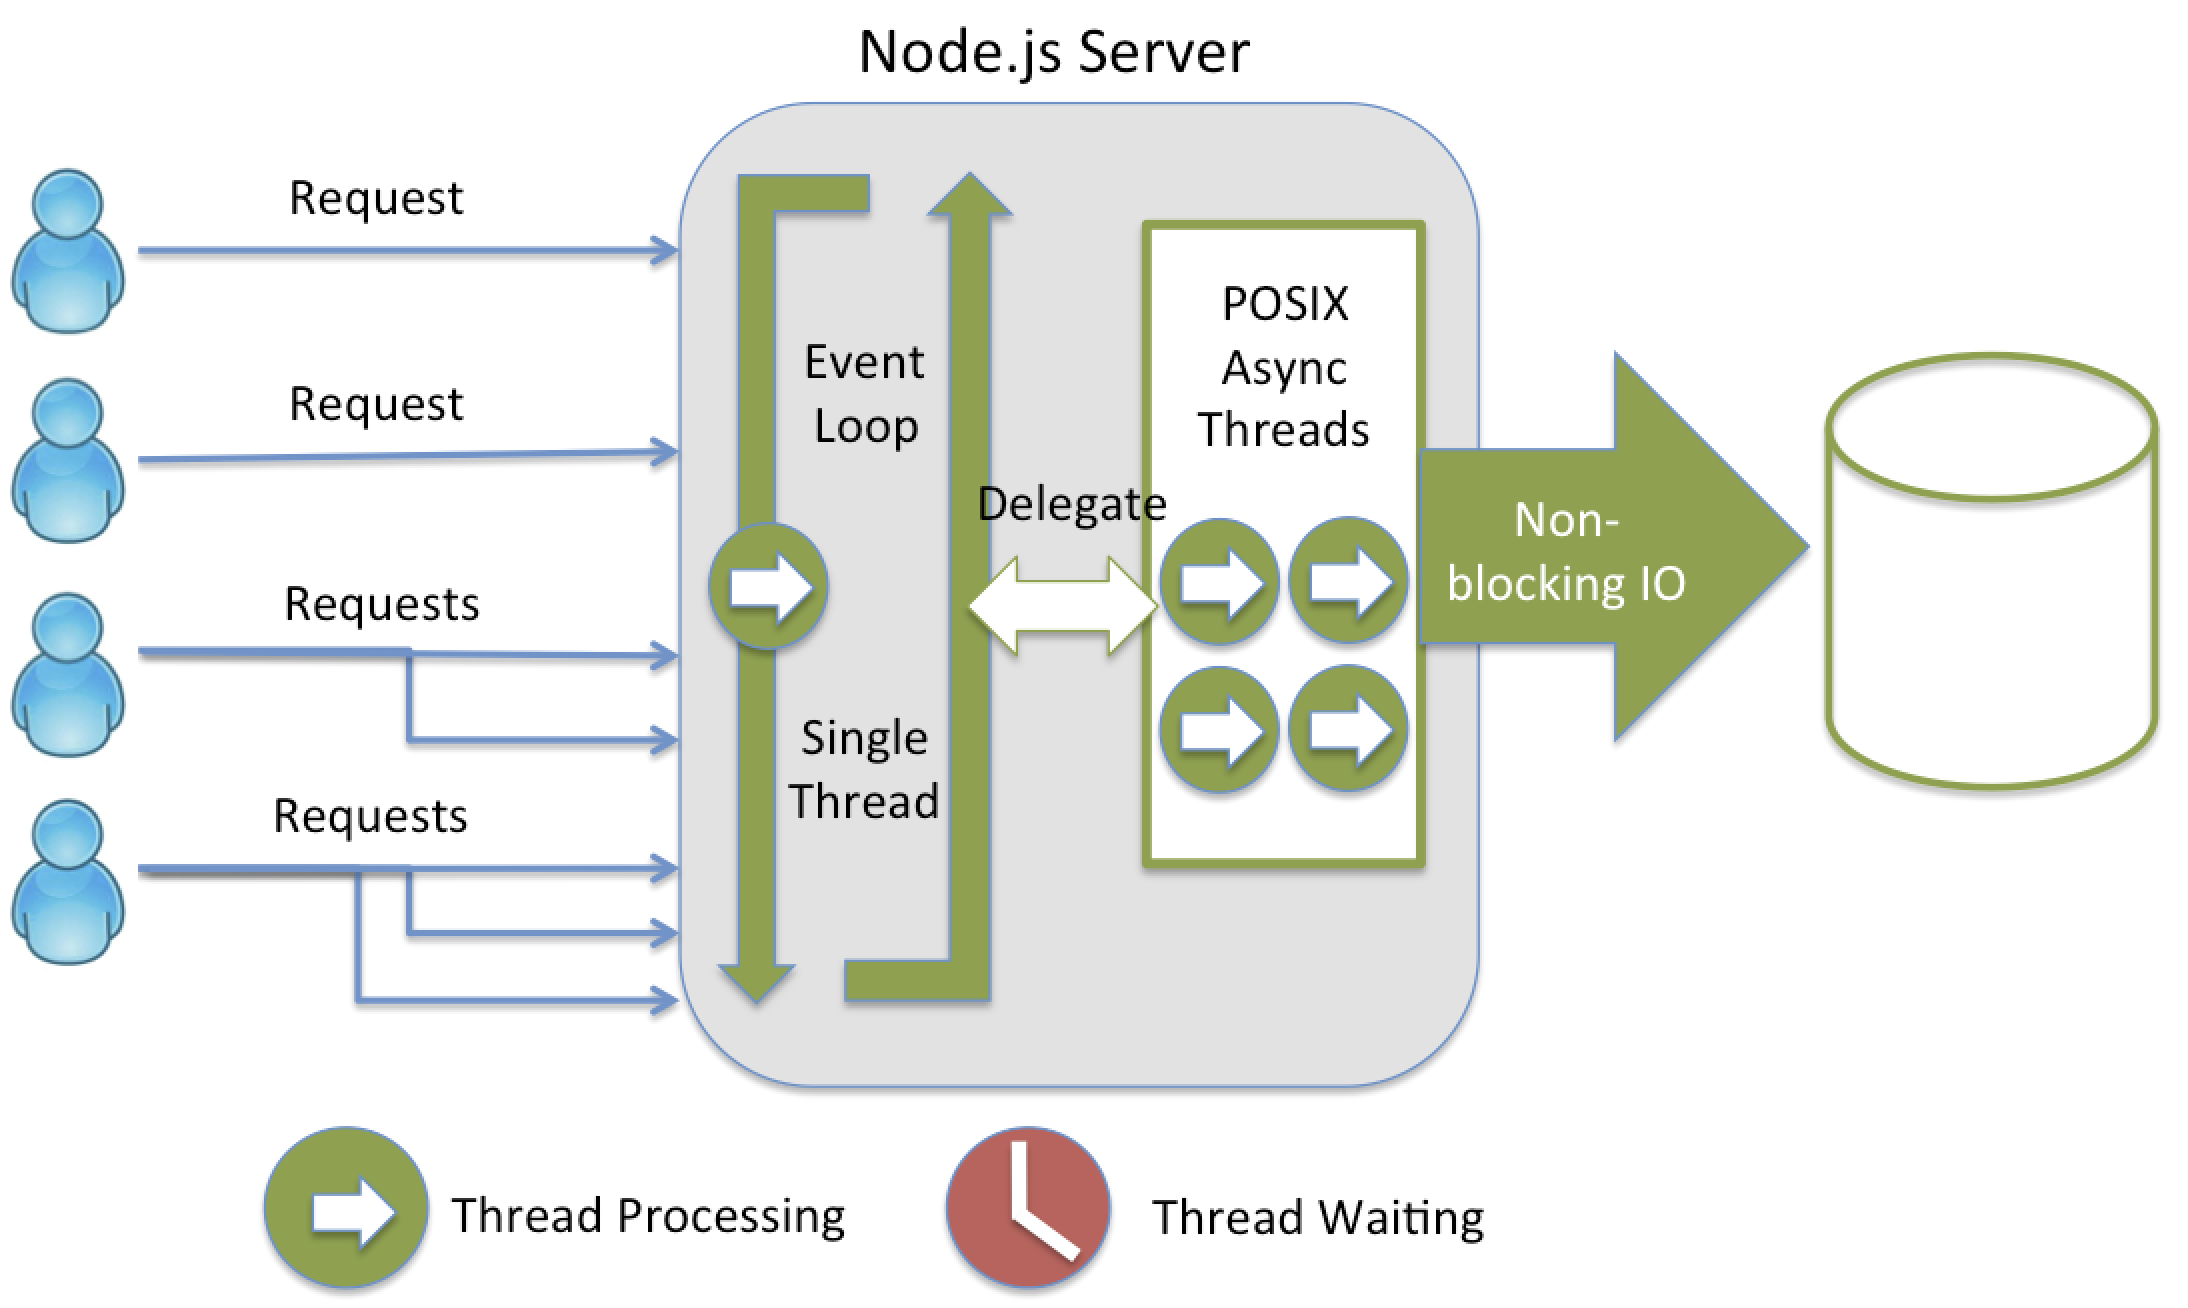
\includegraphics[width=0.6\textwidth]{figures/node.png}
\caption{NodeJS's event driven achitecture.\label{fig:node}}
\end{figure}

\section{Dependent modules}

Using the NPM (Node Package Manager) new dependent packages can be easily downloaded from a central  repository. NodeJS has a great coverage of packages, people can easily share their own modules. It contained 143 300 packages at the time of writing. In the implementation of the monitoring application there was a need for an interface for the database communication, interface for generating the web services and serving web pages. The most important packages were the following: 
\begin{itemize}

\item The ExpressJS module acts as the Servler engine for JavaScript. It handles incomming connections and parsed HTTP request are passed to a callback function which generates the responses. Different urls can have different callback functions to do routing. Express also supports many templating engines, like EJS or JADE.

\item Restler is an easy to use module that can asynchronously read a web page and parse it as JSON data and return it to the callback function. This can be used to communicate with the SOS server as it has an interface that is using JSON post requests to 
receive queries.

\item Stardog.JS is Stardog database servers own connector to get SPARQL queries. It is in early stages, however all the necessary functions are working. 

\item Nodemon, Forever or PM2 are utilities that run NodeJS codes automatically, restarts them on error or code changes. There is a support for development, that on any sourcecode change the changes are pushed to the browser without the need to refresh the browser. They can be configured to restart on error.
\end{itemize}

\section{AngularJS: frontend of the monitoring application}

The ExpressJS module is serving the static files from the backend. The webpage itself is a single page web application which means that it consists of one HTML page and some partial pages that are loaded on the client side by a JavaScript framework. The framework that loads the different modules is called AngularJS. It was acquired by Google and now the project is maintained by them\cite{angular}. It's main advantage is that it implements a clear Model-View-Controller pattern. It dynamically changes the views, the HTML page based on the changes in the model, without additional coding.
It is using dependency injection to be easily extensible.

For manipulating the user interface some external packages has been added to Angular. The most important of those are the following:
\begin{itemize}
\item \textbf{Chart.js}: This is a module that can be used to draw line charts or other kind of charts. This has an Angular integration and can be used to display the measured data in a time series plot. It can automatically smooth the curves. This is an open source project using HTML5.
\item \textbf{Angular Bootstrap DateTime picker}: This module has been chosen to select the time period to display. This is an open source project too.
\item \textbf{NG Tags Input}: This module can display tags in a search box and can handle autocomplete. 
\end{itemize}

For formatting the page the Bootstrap template is used. 
This library has some built in styles that are displayed the same in every browser. It has support for mobile devices. This framework and Angular itself helped in making the application a responsive, mobile friendly application.

There are different building blocks for AngularJS. Those blocks that have been used as part of the development are the following:
\begin{itemize}
\item \textbf{Module} is the main building block of Angular. It is paired to the HTML page and this invokes controllers based on the location provided. The global dependencies are injected into the module and they are inherited by the controllers afterwards.
\item \textbf{Controller} pairs the view to the models. They modify and view according to the model and they load the model if needed. The controller does that using the \$scope global variable, which is shared with the views. The controller sets the template of the inner content(dynamic part) of the web page too.
\item \textbf{Directive}'s are custom defined page elements that can be injected in any page. They have their own controller and template. Custom complex UI elements can be directives.
\item \textbf{Filter}'s can be applied to format the view of the model. Filters can do uppercase, lowercase on strings, sorting of array, format currencies, etc. They are an applied function on a given input data.
\end{itemize}

\section{RDF representation of the SOS data}

\begin{figure}[h]
\centering
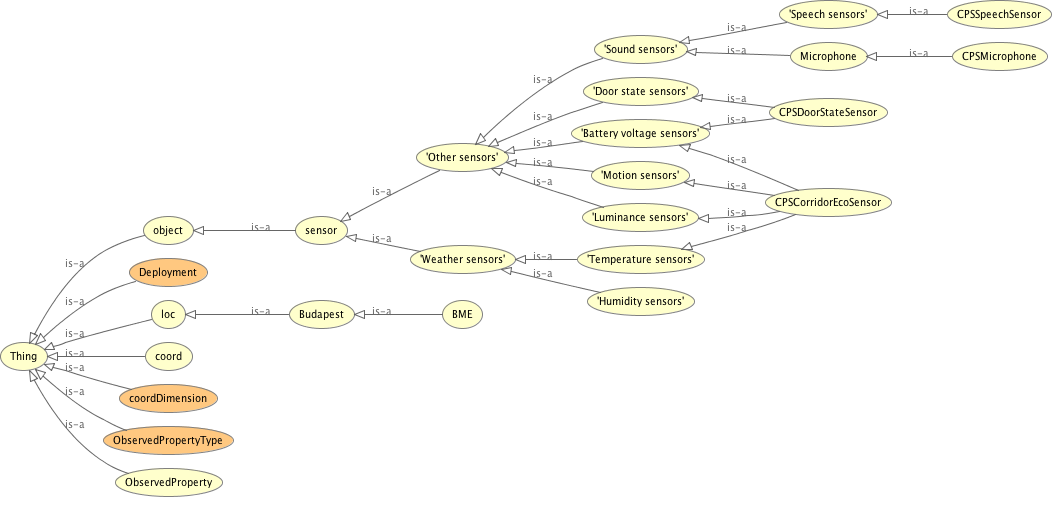
\includegraphics[width=0.9\textwidth]{figures/implrdf.png}
\caption{The Ontology used in the monitoring system.\label{fig:implrdf}}
\end{figure}

The general SISRO representation was missing some data of the example use case at the time of writing. To bridge this problem the monitoring application is using a different ontology that has been created to enable sensor browsing. This ontology contains only the necessary information to query sensor information. The elements can be seen on Figure \ref{fig:implrdf}. Some parts of the ontology hasn't been used in the monitoring system, the key components are:

\begin{itemize}
\item \textbf{Sensor}: This object is the ancestor of all sensor types. It has the Weather and Other sensors and their children. The instances of the child classes are the actual sensors. Figure \ref{fig:implrdf} shows that a final sensor can have multiple measurement, thus it can have multiple parents. Eco sensors are instances of the CPSCorridorEcoSensor and door state sensors are Instances of CPSDoorStateSensors. 
\item \textbf{loc}: This object stores location information, like URI of the feature of interest property in SOS and the name of the location. 
\item \textbf{ObservedProperty}: This is the observed feature of a sensor. There can be multiple observed properties for one sensor, like Battey voltage, Motion sensors, Speech text. The object instance contains the URI for the ObservedProperty in SOS and the type of the observed property.
\item \textbf{ObservedPopertyType}: This is the type of the observed property it has 3 instances in the example application: quantity, text, boolean.
\end{itemize}
 
The sensors of the use case are introduced in the end of the previous chapter, so those won't be covered here in details.
  
\section{Architecture of the monitoring system}

\begin{figure}[h]
\centering
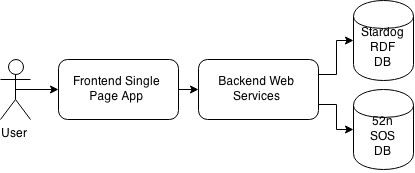
\includegraphics[width=0.6\textwidth]{figures/softwareArch.png}
\caption{Overall architecture of the monitoring system.\label{fig:overallarch}}
\end{figure}

The overall architecture can be seen on Figure \ref{fig:overallarch}. The user communicates through the single page web application. The web application dynamically loads the elements by sending requests to the backend service. The backend service connects to the two different databases and returns the data to the frontend. Initially the client side pages are also served by the backend service. 

\section{Backend web service}

The backend services are called using HTTP POST and GET request. The POST body is always a JSON object. The detailed architecture of the backend services can be seen on Figure \ref{fig:backarch}.


\begin{figure}[h]
\centering
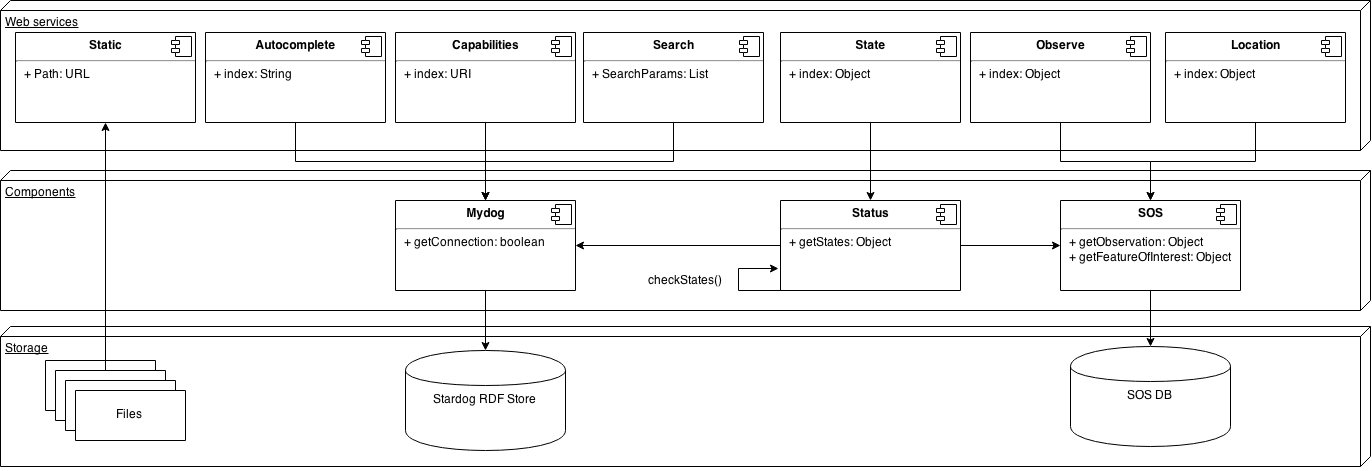
\includegraphics[width=0.9\textwidth]{figures/backendarch.png}
\caption{Detailed architecture of the backend services.\label{fig:backarch}}
\end{figure}

\subsection{Serving static files}
As the backend service is also providing the basic web server features, it has a built in static module, which in case there is no other web service by the provided location, it is serving a file from a given folder. If the file specified in the location does not exist the default index.html is returned. 
This ensures that Angular's custom routes are redirected to the same page. This feature is provided by ExpressJS.

\subsection{Autocomplete service}
In the sensor browser page, there is a search module where you can start typing in the name of the wanted category. After 3 letters a query is sent to the Autocomplete backend service which tries to find the matching categories and returns a list of the result. The Autocomplete service is using the Mydog module to get the data from Stardog. 
The query searches for every descendant of the sensor class and returns the result if found. The SPARQL query for that can be seen on Listing \ref{lst:autosparql}. 
\begin{lstlisting}[caption={SPARQL query for Autocomplete on the "wea" string\label{lst:autosparql}}]
SELECT ?name ?label {?name rdfs:subClassOf+ mit:sensor ; rdfs:label ?label. FILTER regex(?label, "wea","i")}';
\end{lstlisting}

\subsection{Capabilities service}
The Capabilities service receives a procedure and returns all the information that describe the sensor in some way. This is similar to what SOS getCapabilities would return but with additional information. It is done using SPARQL in the RDF store. The result of this service call is used in other parts of the application. The SPARQL query for this can be seen on Listing \ref{lst:capsparql}. The result will be given as a JSON object. It will contain the sensor name, the procedure name, the offering of the procedure, the feature of interest of the procedure, the label of the feature of interest, the observed property URI, its name, and the name of the type of the observed property. 


\begin{lstlisting}[caption={SPARQL query for Capabilities\label{lst:capsparql}}]
SELECT ?label ?procedure ?offering ?foi ?flabel ?observable ?obs_name ?tlabel 
WHERE { <procedure/name> demo:procedure ?procedure ;
 rdfs:label ?label;
 demo:offering ?offering;
 demo:observedProperty ?obs ; 
 mit:hasLoc ?loc.
?loc demo:foi ?foi;
 rdfs:label ?flabel. 
?obs demo:observedPropertyURI ?observable ;
 rdfs:label ?obs_name ; mit:hasObservedPropertyType ?type .
?type rdfs:label ?tlabel}
\end{lstlisting}

\subsection{Search service}
The search service filters the sensor list. By default it will return the list of all sensors in the system. If there is an additional parameter list given in a given format the system will modify the query accordingly. This format is an array of  JSON objects which have three fields: 
\begin{itemize}
\item[text] The displayed name of the given parameter, it is not used in the backend.
\item[value] The class URI which identifies the class itself. This is added to the query.
\item[type] The type of the parameter. Yet it can have the value of "sensortype" only. This may contain additional values if new features provide more conditions for filtering. 
\end{itemize}
The SPARQL query for retrieving the objects can be seen on Listing \ref{lst:searchsparql} The example SPARQL is using two categories for filtering. The result is always the union of the given categories. 

\begin{lstlisting}[caption={SPARQL query for Search\label{lst:searchsparql}}]
SELECT ?procedure ?name ?offering
    { ?class rdfs:subClassOf+ mit:sensor  .
     ?procedure rdf:type  ?class ; rdfs:label ?name ; demo:offering ?offering 
     { ?class rdfs:subClassOf* <category_one> } UNION { ?class rdfs:subClassOf* <category_two> }
    }
\end{lstlisting}

\subsection{Observe service}
The Observe service queries sensor observations and returns them to the frontend.
The time range can be given to the query allowing the frontend to narrow down the data to a manageable level. The service uses the SOS component. It is expecting an object similar to the result of the Capabilities service as an input parameter, and also two datetime strings in ISO 8601 format, which are the start and end times of the observations. The service automatically decreases the number of results to a displayable number of 50 results if more has been found. The result will be two array and some metadata: one array for the date (x field) and another array for the measurements (y field). Boolean results are automatically converted to a series of zeros and ones. The text fields are returned as string values in the y array.

\subsection{Location service}
The Location service queries only the positions of the given object. The object should be given in a format similar to the result of the Capabilities service. The service uses the SOS component to query the featureOfInterest's position and return it as an object. Yet, it can only retrieve point like sensors.

\subsection{State service}
This service retrieves the current status of the system. The status is queried by the Status component from time to time. The service is simply returning the result in a response and some additional metadata about showable fields.

\section{Backend components}
There are three main components for the monitoring system. They all provide needed functionalities the the web services describe before to shae some common tasks.

\subsection{SOS component}
This component provides connectivity to the SOS server. Connection parameters are given in the global config file. The component has two main functions:
\begin{itemize}
\item \textbf{getObservation} queries the SOS database for the result objects in a given timerange for the given sensor.
\item \textbf{getFeatureOfInterest} gets the location of a given sensor and sends it back as an object.
\end{itemize}
The component handles connections using the Restler Node module, which has JSON POST request capabilities.

\subsection{MyDog component}
This component gives helper functions for communicating with the Stardog RDF store. It has one important method, the getConnectin function, which returns a connection to the Stardog database. It has one boolean parameter which is set to true if reasoning functionality is needed in Stardog. The queries are put together in the services themselves. There are some additional helper variables, like the list of prefixes for the SPARQL queries and the database name that is used for the semantic store. Stardog database related settings are also stored in the global configuration.

\subsection{Status component}
This component handles  the status updates for the sensors. Yet it is only prepared to handle small number of sensors for the special use case. The module starts when the whole system starts. 
In a given interval specified in the configuration file it will query all the sensors in the system using the MyDog RDF store and the query on Listing \ref{lst:statussparql}.
After that it is going through all the possible devices and reads observations using the SOS component in the past given period. This period can be set in the global configuration too. 
If there is no data in the given period the sensor is said to be down, otherwise the sensor is marked as up. The current state is maintained in the modules states array. If there has been a change an event can be triggered.
\begin{lstlisting}[caption={SPARQL query for querying all sensors\label{lst:statussparql}}]
SELECT ?procedure ?name ?offering ?foi ?observable ?obs_name ?obs 
    { ?class rdfs:subClassOf+ mit:sensor  .
     ?procuri rdf:type  ?class;demo:procedure ?procedure ; rdfs:label ?name ; demo:offering ?offering;  demo:observedProperty ?obs ; mit:hasLoc ?loc.
     ?loc demo:foi ?foi. ?obs demo:observedPropertyURI ?observable ; rdfs:label ?obs_name ; mit:hasObservedPropertyType ?type .
     ?type rdfs:label ?type_label}
\end{lstlisting}

\section{Components of the frontend}

The frontend is using the mentioned AngularJS framework to provide responsive, dynamically changing web pages to the user. The initial entry point is the index.html file which is a standard HTML page extended with Angular functionalities. Used modules, stylesheets and javascripts are partly added dynamically during the build process done by Grunt build system. 
Angular has a built in routing system which can call the needed modules depending on the URL given. Each module has a controller which loads the template of the module (the View). The frontend components can be seen on Figure \ref{fig:frontarch}.


\begin{figure}[h]
\centering
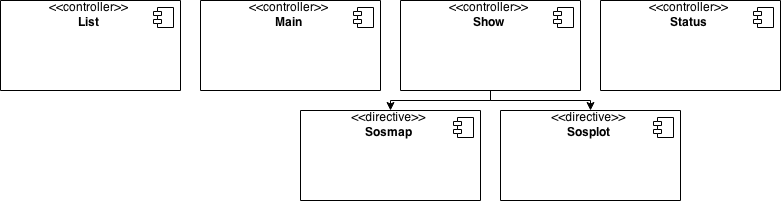
\includegraphics[width=0.9\textwidth]{figures/frontend.png}
\caption{Detailed architecture of the frontend components.\label{fig:frontarch}}
\end{figure}

\subsection{Main component}
The main component renders the opening page with the application help. This page does not have any dynamic property. This is the default route.

\subsection{List component}
This component contains the template to list all the sensors and filter the elements. The template contains a search box directive called ng-taginput which was mentioned before. The filter part uses the backend autocomplete service. The results are loaded using the search backend service. The list is updated every time the filter button is clicked.
The sensor names are clickable and they redirect the users to the show component with the additional procedure parameter. This component can be found on /list route.

\subsection{Status component}

This component lists the result of the periodic status checks. 
It is communicating with the status backend service to get the list and state of the sensors.
There are built in Angular directives that make listing and ordering possible. Some parameters were modified to make custom ordering possible. This component is under the route /status.

\subsection{Show component}

This component accepts one parameter, the identifier of the procedure and shows all the related measurements. It queries the necessary parameters using the capabilities backend service. The service returns all the possible measurements and as a second step it invokes the measurement plotter directive called sosplot for all the possible observable properties.
It also displays the position of the sensor using Google Maps. 
The data date and time range can be selected by a third party datetime AngularJS plugin. After selecting the time the charts are automatically updated. This component highly depends on the two directives Sosplot and Sosmap.

\subsection{Sosplot component}
This component is an Angular directive. These directives act as new custom designed HTML elements, which Angular will transform into standard web page elements. The Sosplot directive is used to display measurement data. It needs three parameters, an object which contains the details of the observed property and the start and end time. Using this information it uses the backend observe service to query the measurements and then display the results using the previously mentioned Chart.JS third party chart plotter module. If the data is not plottable, like if we have text property type, the directive automatically loads a different template that will render a list of the text messages. 

\subsection{Sosmap component}
The Sosmap component is an Angular directive which is using the Google Maps API to display the position of the sensor. The directive is using the location backend service. Now it is capable of displaying single points on a map.

